\documentclass[
        12pt,
        openany, %openright,			
        oneside, %twoside,			%% twoside: para frente e verso ao imprimir
        a4paper,			
        english,			
%	french,				%% Idioma adicional 
%	spanish,			%% Idioma adicional 
        brazil			        %% Idioma principal 
        ]{abntbibufjf}

\usepackage{lmodern}						
\usepackage[T1]{fontenc}		
\usepackage[utf8]{inputenc}		%% Para converter automaticamente acentos como digitados. Mude utf8 para latin1 se precisar. 
                                        %% Permite digitar os acentos no teclado normalmente, sem comandos (\'e \`a , etc.).
\usepackage{lastpage}			
\usepackage{indentfirst}		
\usepackage{color}		
\usepackage[alf,abnt-emphasize=bf,abnt-etal-list=0,abnt-etal-text=it]{abntex2cite}	
\usepackage{graphicx}			
\usepackage{microtype} 	



%% -----------------------------------------------------------------------------

%% Obs.: Alguns acentos foram omitidos.

\titulo{Implementando a metodologia lean no desenvolvimento de software} %%Por exemplo, Titulo da tese
% \subtitulo{: subt\'itulo do trabalho}  %% Retirar o primeiro ``%'' desta linha se for utilizar subtitulo. Deixar os dois pontos antes, em ``: subt\'itulo'' . 
\autor{André Furquim}
\autorR{Furquim, André} %%Colocar o sobrenome do autor antes do primeiro nome do autor, separados por ,
\local{Joinville}
\data{2015} %%Alterar o ano se precisar
\orientador[Orientador:]{Maurício Henning} %%Se precisar, troque [Orientador:] por [Orientadora:]
% \coorientador[Coorientador:]{Nome do coorientador } %% Retirar o primeiro ``%'' desta linha se tiver coorientador. Se precisar, troque por [Cooorientadora:]. 
\instituicao{Centro Universitário -- Católica de Santa Catarina}
\faculdade{Instituto de Ci\^encias Exatas} %%Alterar, dentro de chaves {}, se precisar.
\programa{Curso de P\'os\mbox{-Gra}dua\c{c}\~ao em Engenharia de Software} %%Alterar, dentro de chaves {}, se precisar.
\objeto{Monografia}  %%Tese (Doutorado)
\natureza{Monografia  %%Tese
apresentada ao \insereprograma ~do \insereinstituicao ~como requisito parcial para obten\c{c}\~ao do certificado do curso.} %%Trocar Matem\'atica por outro, se precisar.


%% Abaixo, prencher com os dados da parte final da ficha catalografica

\finalcatalog{1. Lean. 2. Metodologia de Desenvolvimento. 3. Engenharia de Sofware. I. Henning, Maurício. Msc.} %% Aqui fica 
% escrito a palavra ``T\'itulo'' mesmo, nao o do trabalho. Se tiver coorientador, os dados ficam depois dos dados 
%% do orientador (II. Sobrenome, Nome do coorientador, coorient.) e antes de ``II. T\'itulo'', o qual passa a ``III. T\'itulo''.

%% ---

\setlength{\parindent}{1.3cm}

\setlength{\parskip}{0.2cm}  

\setlength\afterchapskip{12pt}  

%% Iniciar o documento
\begin{document}

%% ELEMENTOS PRE-TEXTUAIS

%% Capa
\inserecapa

%% Folha de rosto
\inserefolhaderosto


%% Ficha catalografica. AO IMPRIMIR, DEIXAR NO VERSO DA FOLHA DE ROSTO.
\inserecatalog  


%% Folha de aprovacao
\begin{folhadeaprovacao}

  \begin{center}
    {\chapterfont \MakeUppercase{\bfseries \insereautor}}

    \vfill
    \begin{center}
      {\chapterfont \MakeUppercase{\bfseries\inseretitulo \inseresubtitulo}}
    \end{center}
    \vfill
    
    \hspace{.45\textwidth}
    \begin{minipage}{.5\textwidth}
        \inserenatureza
        \\ \\
        \begin{center}COMISSÃO EXAMINADORA \end{center}
         \assinatura{Prof. Msc. \insereorientador \ - Orientador \\ Centro Universitário -- Católica de Santa Catarina} 
      %  \assinatura{Professor Dr. \inserecoorientador \ - Coorientador \\ Universidade Federal de Juiz de Fora}
         \assinatura{Prof. }
         \assinatura{Prof. } 
    \end{minipage}%
    \vfill
   \end{center}
           

%  \assinatura{...} %%RETIRE O % E PREENCHA SE PRECISAR
%  \assinatura{...}
%  \assinatura{...}
\end{folhadeaprovacao}


%% Dedicatoria. OPCIONAL. Retirar o ``%'' de cada das 4 linhas abaixo, caso queira.
% \begin{dedicatoria} \vspace*{\fill} \centering \noindent
%   \textit{ Dedico este trabalho ... (opcional)} 
%   \vspace*{\fill}
% \end{dedicatoria}


%% Agradecimentos. OPCIONAL. CASO SEJA BOLSISTA, INSERIR OS DEVIDOS AGRADECIMENTOS.
\begin{agradecimentos}

Este trabalho é decicado à minha família, meus amigos, meu orientador e a Católica de Santa Catarina. 

\end{agradecimentos}

%% Epigrafe. OPCIONAL
% \begin{epigrafe}
%     \vspace*{\fill}
% 	\begin{flushright}
% 		``Texto em que o autor apresenta uma cita\c{c}\~ao, seguida de autoria, relacionada com a                       
%   mat\'eria tratada no corpo do trabalho'' \\
% (ASSOCIA\c{C}\~AO BRASILEIRA DE NORMAS T\'ECNICAS, 2011, p. 2) \\
%   A ep\'igrafe elaborada conforme NBR 10520 (Ep\'igrafe - Opcional)
% 	\end{flushright}
% \end{epigrafe}


%% RESUMOS

%% Resumo em Portugu^es. OBRIGATORIO.
\setlength{\absparsep}{18pt} 
\begin{resumo}
O software como produto foi ganhando cada vez mais importância com o passar do tempo, assim foi necessário investir em modelos que pudessem melhorar seu desenvolvimento para que fosse possível garantir melhor qualidade, custo e prazo no projeto de software. Um modelo que vem ganhando mais notoriedade atualmente é o modelo de desenvolvimento lean, o qual tem seu foco em criar valor para o cliente através da eliminação de desperdícios, otimização do fluxo de valor, capacitação das pessoas e melhora contínua. Esse modelo, criado pela Toyota, embora aplicado em muitas empresas, ainda possui desafios no que tange a sua utilização no mercado de software. Esse trabalho tem como objetivo esclarecer o leitor sobre essa metodologia e apresentar maneiras de como proceder para aplicação da metodologia lean de desenvolvimento em uma empresa de software.

\textbf{Palavras-chave}: Lean, Metodologia de Desenvolvimento de Software, Engenharia de Software. %finalizadas por ponto e inicializadas por letra maiuscula.

\end{resumo}
 
 
%% Resumo em Ingle^s
\begin{resumo}[ABSTRACT]
 \begin{otherlanguage*}{english}
 The software as a product has been growing in terms of importance over the time in people’s life, thus it's necessary to invest in models in order to improve software development in the sense of guaranteeing a better quality, cost and time in a software project. A model that has been growing in importance over the software community is lean, which focuses on creating customer value through waste elimination, value stream optimization, people empowerment and continuous improvement. Although this model, created by Toyota, is widely applied in several companies, it’s still a challenge regarding to software market. This work aims to explain the reader about this methodology and present ways to implement lean in a software company.

\textbf{Keywords}: Lean, Software Development Methodology, Software Engineering.
 \end{otherlanguage*}
\end{resumo}

%% Seguindo o mesmo modelo acima, pode-se inserir resumos em outras linguas. 

%% Lista de ilustracoes. OPCIONAL.
\pdfbookmark[0]{\listfigurename}{lof}
\listoffigures*
\cleardoublepage


%% Lista de tabelas. OPCIONAL. Retire o ``%'' de cada das 3 linhas seguintes, caso queira.
\pdfbookmark[0]{\listtablename}{lot}
\listoftables*
\cleardoublepage

%% Lista de abreviaturas e siglas. OPCIONAL
\begin{siglas} %%ALTERAR OS EXEMPLOS ABAIXO, CONFORME A NECESSIDADE
  \item[AWS] \textit{Amazon Web Services}
  \item[BDD] \textit{Bevavior Driven Development}
  \item[DSDM] \textit{Dynamic Systems Development Methodology}
  \item[FDD] \textit{Feature Driven Development}
  \item[GQM+] \textit{Goal Question Metric}
  \item[IHC] Interface Humano Computador
  \item[JAD] \textit{Joint Application Design}
  \item[JIT] \textit{Just in Time}
  \item[LSD] \textit{Lean Software Development}
  \item[PSP] \textit{Personal Software Process}
  \item[SAAS] \textit{Software as a Service}
  \item[RUP] \textit{Rational Unified Process}
  \item[TDD] \textit{Test Driven Development}
  \item[TSP] \textit{Team Software Process}
  \item[UAP] \textit{Unified Agile Process} 
  \item[UML] \textit{Unified Modeling Language}
  \item[XP] \textit{Extreme Programming}
\end{siglas}

%% Lista de simbolos. OPCIONAL
% \begin{simbolos} %%ALTERAR OS EXEMPLOS ABAIXO, CONFORME A NECESSIDADE
%   \item[$ \forall $] Para todo
%   \item[$ \in $] Pertence
%  \end{simbolos}

 
%% Sumario
\pdfbookmark[0]{\contentsname}{toc}
\tableofcontents*
\cleardoublepage

%% ----------------------------------------------------------

%% ELEMENTOS TEXTUAIS

\textual
\pagestyle{simple}   

\setcounter{page}{1}
\chapter{INTRODU\c{C}\~AO}  %%Nesta linha, dentro de { }, digita-se em CAIXA ALTA, como apresentado aqui
\label{chap:01}
A engenharia de \textit{software} surgiu como um esforço de aplicar processos que pudessem dar maior assertividade nos projetos de \textit{software}. Através desses esforços surgiram vários modelos que contribuíram para melhorar o cenário de desenvolvimento. Pode-se dizer que esses esforços foram também impulsionados através do mercado, o qual se torna cada vez mais competitivo e exige que os projetos de \textit{software} tenham que ser desenvolvidos com extrema qualidade e de forma rápida, repetida e confiável.
Dentre as várias metodologias que surgiram, uma metodologia está ganhando bastante destaque no mercado atual: o \textit{lean}. \citeonline{4222727} aponta que iniciativas \textit{lean} (ou enxuta)\footnote{Neste trabalho é empregado a palavra em inglês lean.}  tem sido utilizadas com sucesso em vários setores como manufatura, logística, serviços e no desenvolvimento de produtos, a fim de garantir uma melhor entrega no que tange ao custo, qualidade e prazo. Uma pergunta que surge naturalmente é: “É possível aplicar os mesmos conceitos já aplicados em outros setores para o \textit{software} ?”. Esse trabalho propõe-se a responder essa e outras perguntas sobre aplicação do \textit{lean} no contexto de \textit{software}.
Na seção seguinte, são mostrados alguns trabalhos na linha de pesquisa do \textit{lean} e que contribuíram para o trabalho.

\section{TRABALHOS RELACIONADOS}

No trabalho  de \citeonline{4222727} é mostrado um breve tutorial para aplicação de \textit{lean} no desenvolvimento de \textit{software}. O \textit{lean} é focado em sete princípios:

\begin{itemize}
	\item Eliminar desperdício;
	\item Incorporar qualidade;
	\item	Criar conhecimento;
	\item	Adiar compromisso;
	\item	Entregar rápido;
	\item	Respeitar pessoas e
	\item	Otimizar o todo.
\end{itemize}

Todo esse grupo de princípios, segundo esse trabalho, fornece uma orientação de como entregar um \textit{software} de forma rápida, melhor e com um custo menor. Neste trabalho é afirmado que o desenvolvimento de \textit{software lean} fornece a teoria por trás das práticas utilizadas pelo desenvolvimento ágil. Além disso, o \textit{lean} fornece para as empresas uma série de princípios para melhorar o processo de engenharia de software com a finalidade de trazer melhora no contexto do cliente, domínio do negócio, capacidade de desenvolvimento e em uma eventual situação única que a empresa enfrente.

Neste trabalho, um tutorial foi feito com uma turma e a aplicabilidade do \textit{lean} no desenvolvimento de \textit{software} é feita através dos seus princípios fundamentais. No princípio do desperdício, além de sua explicação no contexto de \textit{lean}, foi mostrado como enxergar o desperdício no contexto do desenvolvimento e explanado os sete desperdícios no desenvolvimento de \textit{software}. Nesta etapa, a classe foi divida em grupos de até sete pessoas e foi feito um mapeamento de fluxo de valor da experiência de alguém no grupo. Após a elaboração, os grupos apresentaram seu mapa e receberam críticas dos outros participantes.

Para o próximo conceito do \textit{lean}, qualidade, foram apresentados conceitos como: TDD (\textit{test-driven development}), teste unitário automatizado e teste de aceitação. Essa etapa não focou muito em como fazer, mas o porquê da importância dessas práticas para o \textit{lean}\textit{.}

Uma análise racional, no que se refere ao conhecimento, foi feita sobre a questão de postergar os compromissos (princípio do pensamento \textit{lean}). Também foram apresentados métodos que visam preservar o conhecimento de forma que os times não tenham que reaprender o que já foi aprendido. Além disso, foi feita uma discussão dos benefícios da utilização de uma abordagem que envolve explorar múltiplas soluções em vez de focar em apenas uma.

Para questão de velocidade é discutido a aplicação da teoria das filas no desenvolvimento de \textit{software}. Nela foi mostrado o porquê de longas filas serem prejudiciais ao desenvolvimento e mostrado como evita-las. Além disso, é mostrado que ciclos de vida rápidos tendem a dar uma qualidade maior ao projeto de \textit{software} e reduzir seu custo.

Por fim, foi discutido a importância de enxergar um sistema como um todo. Através dessa discussão foi explanado que não é suficiente focar apenas no desenvolvimento em si, assim foi mostrado como mudar o foco do desenvolvimento para os esforços dos objetivos em geral, ou seja, o produto ou o processo apoiado pelo \textit{software}. 

A abordagem de migração para o \textit{lean} de uma empresa de \textit{software}, no trabalho de \citeonline{7107412}, também foi feita a partir da medição do fluxo de valor da organização com posterior utilização desses dados para migração. Essa equipe já utilizava a metodologia ágil de desenvolvimento. Para medir o fluxo de valor, são medidos aspectos de interesse das atividades, recursos utilizados e artefatos produzidos. É importante notar que, como assinala \citeonline{7107412}, o que é de interesse do ponto de vista para os objetivos de uma empresa não necessariamente é para outra. Por isso é utilizado a estratégia GQM+ (\textit{Goal Question Metric Plus}). A estratégia GQM+ é uma nova abordagem de medida baseada no GQM (\textit{Goal Question Metric}). A diferença segundo \citeonline{DBLP:journals/corr/BasiliHLMRRST14} é que o GQM+ alinha as medidas do \textit{software} com os objetivos da empresa. Essa abordagem foi necessária a fim de ajudar na correspondência das estratégias com a necessidade de informação e medidas. Os dados obtidos são usados para entender melhor o processo de desenvolvimento de \textit{software}. Uma técnica chamada Andon é então utilizada no sentido de fornecer um mecanismo para visualização dos dados por qualquer pessoa com o menor esforço possível. Através desse mecanismo de visualização, um feedback para o time é feito no sentido de guia-los nos seus objetivos. Na figura \ref{fig:01} é mostrado um mapa que ilustra a dinâmica do \textit{lean} em uma empresa que emprega o processo de desenvolvimento ágil.

\begin{figure}[hb]
\begin{center}
\caption{Mapas de conceito descrevendo os blocos de construção do desenvolvimento de software lean}
\label{fig:01}
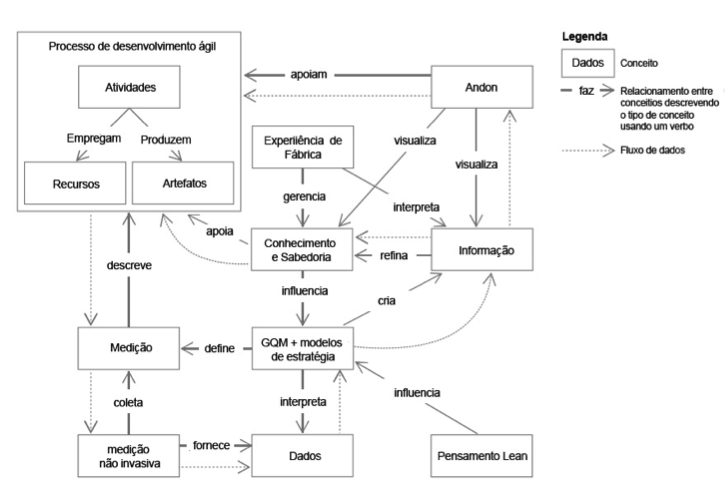
\includegraphics[width=15cm]{assets/figura1} \\
\fonte{Adaptado de \citeauthoronline{7107412}, \citeyear{7107412}.}
\end{center}
\end{figure}

Na Figura \ref{fig:01} obverva-se que o processo de desenvolvimento ágil possui atividades, as quais utilizam-se de recursos e produzem artefatos. É possível perceber também que o processo do \textit{lean} não está associado unicamente ao processo de desenvilmento da organização. Por essa razão a abordagem GQM+ foi um diferencial. Através de um sistema de retroalimentação, tem-se um \textit{feedback} que contribui também para melhora contínua do sistema como um todo.

O trabalho de \citeonline{6005500} foca na combinação do \textit{lean} com metodologias ágeis, como o trabalho de \citeonline{7107412}. \citeonline{6005500} afirma que existem linhas de pesquisa que consideram que ágil e o \textit{lean} são dois nomes para mesma coisa, enquanto outras linhas consideram que não. Os autores que consideram que \textit{lean} e ágil não são a mesma coisa possuem basicamente duas visões: a de que \textit{lean} e ágil estão em níveis diferentes dentro da organização e outra que afirma que \textit{lean} e ágil possuem diferentes focos e escopos. \cite{6005500}

% Para algumas linhas de pesquisa, as duas metodologias tem o mesmo objetivo, mas estratégias diferentes. O \textit{lean} nasceu de uma filosofia de gerenciamento que foca nos seus princípios, e.g. eliminação de atividades que não agregam valor ao cliente, não apenas dentro do gerenciamento da organização como em toda cadeia (o que inclue o desenvolvimento). Nesse sentido, pode-se afirmar que sua aplicabilidade dentro da organização segue uma abordagem \textit{top-down}, ou seja, de cima para baixo (gerenciamento para o operacional). Em contrapartida ao \textit{lean}, o ágil nasceu como uma filosofia de metodologia de desenvolvimento, ou seja, já nasceu como uma abordagem que empregava ideias concretas que focam em atividades que agregam valor no produto, como é o caso do \textit{lean}, mas que promovem uma mudança na organização de baixo para cima.



Para visão de que \textit{lean} e ágil estão em diferentes níveis dentro da mesma organização, é utilizado o pensamento \textit{lean} como um guia de princípios para desenvolver e aplicar práticas ágeis. Assim, são propostos sete princípios que são traduzidos para práticas ágeis no contexto do desenvolvimento de um \textit{software}. Para outra visão, que considera que as metodologias possuem focos e escopos diferentes, métodos ágeis estão apenas preocupados com a prática de desenvolvimento e com o gerenciamento do projeto, deixando de lado o contexto global ou de negócio. Nesse sentido, o \textit{lean} se diferenciaria na questão de sua aplicação do escopo, que pode ser desde uma prática de desenvolvimento até uma empresa inteira, onde o desenvolvimento é apenas uma parte do sistema. \cite{6005500}

Considerando que \textit{lean} e ágil são diferentes, pode-se ter várias combinações possíveis de \textit{lean} em uma empresa. Essas combinações serão vistas mais adiante no trabalho e escolhidas para o contexto do estudo de caso.

%A abordagem \texit{top-down}, 

%Para \citeonline{6005500}, alguns autores afirmam que o \texit{lean} é uma filosofia ou um conjunto de princípios, enquanto que o ágil está associado mais ao nível prático. Assim, esses princípios do \textit{lean} são verdades que não mudam com o tempo e espaço, enquanto que as práticas são as aplicações de um princípio para uma situação particular e devem ser diferentes de um ambiente para o outro (mundando conforme o sistema como um todo evolui). Nesse sentido, o pensamento \textit{lean} é utilizado como um guia de princípios para desenvolver e adaptar as práticas ágeis. Outra linha de pesquisa considera que o \textit{lean} e ágil tem escopo e foco diferentes. Assim, o ágil está mais preocupado com práticas de desenvolvimento e gerenciamento de \textit{software} que norteiam o desenvolvimento (deixando de lado o contexto do negócio). Baseado nessas diferenças conceituais, o trabalho propõe maneiras de combinar as duas metodologias em uma organização.

Na seção seguinte são abordados os objetivos geral e específicos deste trabalho.

\section{OBJETIVOS}
\label{chap1:obj}
O objetivo deste trabalho é propor uma metodologia de aplicação do \textit{lean} em uma empresa de \textit{software} que já utiliza-se de algumas práticas ágeis. Assim, é necessário identificar pontos falhos no modelo de desenvolimento da empresa para melhorar os projetos.

Para elaborar esse modelo, algumas perguntas precisam ser antes respondidas como:

\begin{itemize}
	\item Como aplicar \textit{lean} no ambiente de desenvolvimento ?
	\item Existe uma formula que possa ser aplicada para qualquer empresa ?
	\item O quanto as práticas atuais da empresa estão perto ou longe do melhor cenário possível para o \textit{lean} ?
	\item Quais ferramentas de \textit{software} podem auxiliar o processo ?
\end{itemize}

Ao longo desse trabalho, essas perguntas são respondidas.

\subsection{Objetivos Específicos}

Afim de melhorar o ciclo de desenvolvimento, é necessário eliminar os desperdícios (um dos princípios do \textit{lean}). Assim é necessário:

\begin{itemize}

\item representar o modelo atual de desenvolvimento de uma maneira que fique bem claro para as pessoas envolvida, tanto a nível de negócio como operacional, os problemas existente; 

\item Propor um novo modelo, que elimine esses desperdícios e

\item Sugerir ferramentas que possam melhorar o processo de desenvolvimento.

\end{itemize}


% VOLTAR AQUI PARA ATUALIZAR UMA REFERENCIA DEPOIS
\section{CONCLUSÃO DO CAPÍTULO}

Esse capítulo teve como objetivo abordar o \textit{lean} de forma superficial. Foi visto que há autores que consideram que \textit{lean} e ágil são dois nomes para mesma coisa e autores que consideram que não. Os autores que consideram ágil e \textit{lean} como coisas distintas possuem basicamente duas visões: que eles focam em nível diferentes dentro da empresa e outra que eles possuem foco e escopos diferentes. Além disso, foi proposto como trabalho uma maneira de melhorar um modelo de desenvolvimento de \textit{software} em uma empresa. Mais detalhes são fornecidos no Capítulo 4. No Capítulo \ref{cap:02} é feita uma breve revisão dos modelos de desenvolvimento, alguns ainda utilizados e outros não pelas empresas a fim de contextualizar a evolução da contrução de \textit{software}.

\chapter{NOME DO CAP\'ITULO}

Texto do segundo cap\'itulo.


%% ----------------------------------------------------------

%% ELEMENTOS POS-TEXTUAIS
\chapter{LEAN SOFTWARE DEVELOPMENT}
\label{cha:lean}

Não é possível falar do desenvolvimento de \textit{software} enxuto (ou \textit{lean software development}) sem antes falar do sistema de produção criado pela Toyota e que deu origem ao \textit{lean}. Esse capítulo tem como objetivo aprofundar o leitor sobre a metodologia \textit{lean} de desenvolvimento de \textit{software} e dar uma introdução de seu surgimento na manufatura até sua utilização no desenvolvimento de \textit{software} conforme \citeonline{poppendieck:07}.
\label{lean}
\section{INTRODUÇÃO}

O sistema Toyota de produção, que deu origem ao \textit{lean}, surgiu como uma alternativa ao modelo de produção em massa aplicado por Henry Ford em 1914. Henry Ford conseguiu, através da produção em massa, aumentar o salário de 2,4 dolares por 9 horas de trabalho para 5 dolares por 8 horas de trabalho diário. Tudo isso foi conseguido através da redução de 85\% do trabalho sobre a produção do carro e da redução de 12 horas para apenas 90 minutos na sua produção, a qual passava através de uma linha de montagem com trabalho especializado. Nenhum trabalhador precisava saber fazer um carro inteiro, sendo necessário apenas treinar o funcionário para executar um tipo de trabalho na linha de produção. No sistema fordista de produção, o trabalho passou a ser essencialmente especializado e feito por qualquer tipo de pessoa, que poderia ser subtituída facilmente. Esse sistema de produção em massa demonstrou ser viável durante um certo tempo, mas apresentou problemas como a dificuldade de adaptação do modelo em relação a complexidade, que pode ser corroborada pela seguinte frase atribuída a Ford: ``O cliente pode ter o carro da cor que quiser, contanto que seja preto''. No modelo de produção em massa, o custo de uma mercadoria é reduzido de 15\% até 25\% conforme o número de unidades dobra, porém o custo de produção sobe de 20\% para 35\% cada vez que a variedade dobra.

O sistema de produção da Toyota apresenta vários conceitos e ideias que possibilitaram melhorar o sistema de produção e deixar as empresas mais competitivas como o fluxo JIT (\textit{Just in Time}) e o Jidoka (Autonomia). O fluxo JIT nada mais é do que eliminar o estoque e repensar o processo de produção em pequenos lotes. De modo prático, no sistema fordista tinha-se uma máquina especializada em fazer apenas uma peça do carro em massa, já no sistena da Toyota uma máquina poderia ser adaptada rapidamente para fazer diferentes partes rapidamente. O Jidoka, ou autonomia implantou a ideia de qualidade, fazendo com que qualquer evento anormal no processo de produção fizesse com que a produção fosse interrompida automaticamente, o que eliminava desperdício. O sistema deve ser projetado então para ser a prova de falhas, sem necessidade de um humano testando ou supervisionando para detectar erros, ou seja ele é isento de inspeção.

\section{LEAN}

A palavra \textit{lean}, empregada hoje, foi resultado da nova atribuição dada pelo livro lançado em 1990 e entitulado \textit{The Machine That Changed The World} para o que era chamado de JIT (\textit{Just-in-Time}) ou sistema Toyota de produção. Depois de seu lançamento, o que antes era chamado de sistema de produção Toyota passou a ser chamar produção enxuta ou \textit{Lean Production}. No início houve muita aversão ao emprego desse novo modelo de produção, mas conforme o tempo passou o pensamento \textit{lean} atingiu sucesso e foi empregado da manufatura para outras  áreas como: cadeia de suprimentos, desenvolvimento de produtos e no desenvolvimento de \textit{software}. A Figura \ref{fig:lean_tree} mostra a extensão do modelo \textit{lean} para outras áreas através da árvore da família \textit{lean}.

\begin{figure}[htb!]
\begin{center}
\caption{Árvore da família \textit{lean}}
\label{fig:lean_tree}
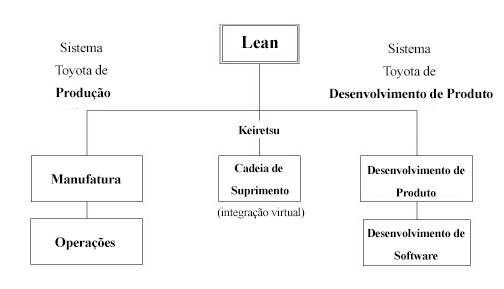
\includegraphics[width=11cm]{assets/lean_tree} \\
\fonte{\citeauthoronline{poppendieck:07}, \citeyear{poppendieck:07}.}
\end{center}
\end{figure}

Na área de manufatura, por exemplo, há o exemplo da companhia Dell de computadores que consegue entregar computadores customizáveis dentro de poucos dias. No que tange a cadeia de suprimentos, não adianta uma empresa ser \textit{lean} se os fornecedores da qual ela depende não forem. No exemplo da Dell, as empresas envolvidas na cadeia de produção do computador aprendem como trabalhar além da fronteira da empresa para alinhar seus interesses com a cadeira inteira de suprimentos. A manufatura enxuta e desenvolvimento enxuto compartilham certas características, o que torna fácil seu emprego no desenvolvimento de produto como redução no tempo de manufatura e redução no tempo de desenvolvimento. O \textit{software} nada mais é do que o desenvolvimento de um produto, sendo o desenvolvimento apenas um subconjunto de todo o processo. Nesse sentido, não há como melhorar a capacidade de desenvolvimento sem melhorar e entender o que constitui o desenvolvimento eficaz de um produto. Por isso, os princípios que regem o sistema Toyota de produção e o sistema Toyota de desenvolvimento são os mesmos. Os princípios do \textit{lean} para o desenvolvimento de \textit{software} são vistos a seguir.

\section{OS PRINCÍPIOS DO \textit{LEAN} NO DESENVOLVIMENTO}

A seguir são vistos os princípios do \textit{lean} no contexto do desenvolvimento de \textit{software} que são: 

\begin{itemize}
	\item Eliminação de desperdício;
	\item Incorporar qualidade;
	\item Criar conhecimento;
	\item Adiar compromisso 
	\item Entregar rápido
	\item Respeitar as pessoas e
	\item Otimizar o todo.
\end{itemize}

\subsection{Eliminação de Desperdício}
\label{sec:desperdicios}
O princípio da eliminação de desperdício é relacionado a tudo que não agrega valor para o cliente. No desenvolvimento de \textit{software} é importante entender o que significa esse valor, o qual pode mudar pelo fato dos clientes nem sempre saberem o que querem. Após entender esse desperdício, é preciso saber enxergá-lo dentro da organização. No desenvolvimento tudo que interfere no sentido de impedir que os usuários recebam esse valor ou qualquer atraso para que isso ocorra é considerado desperdício. Um exemplo comum de desperdício no desenvolvimento são funcionalidades extras. Segundo \citeonline{poppendieck:07} apenas 20\% das funcionalidades extras são usadas regularmente. Essas funcionalidades são basicamente coisas que não foram planejadas no início do desenvolvimento, mas que fazem com que a complexidade e manutenção do código se tornem custosa (além de testes desnecessários). Numa situação como essa, a empresa pode estar potencialmente gastando bastante com suporte e manutenção de funcionalidades que não agregam valor, ao invés de investir em coisas realmente úteis. Um mito que existe no desenvolvimento é que quanto mais cedo a especificação ocorrer, menor será o desperdício. Isso não é verdade, especialmente porque o cliente quase sempre não sabe o que precisa. Um escopo de funcionalidades que o sistema potencialmente pode ter pode ficar extenso e sofrer bastante modificações. 

A real motivação por trás da emilinação de desperdício é descobrir e eliminar desperdícios que podem reduzir custos e tornar os produtos mais efetivos. A Tabela \ref{tab:desperdicio} mostra a equivalência dos desperdícios na manufatura e no desenvolvimento de \textit{software}. Mais abaixo, é descrito um pouco sobre cada um desses desperdícios.

\begin{table}[htb!]
\centering
\caption{Os Sete Desperdícios}
\label{tab:desperdicio}
\vspace{0.5cm}
\begin{tabular}{l|l}

\hline                                
\textbf{Manufatura} & \textbf{Desenvolvimento de Software} \\ 
\hline                               
Estoques no processo & Trabalho parcialmente realizado \\
Superprodução & Funcionalidades extras \\
Excesso de Processamento & Reaprendizagem \\
Transporte & Transferência de controle \\
Movimentação & Troca de Tarefas \\
Esperas & Atrasos\\
Defeitos & Defeitos \\                               
\end{tabular}
\fonte{\citeauthoronline{poppendieck:07}, \citeyear{poppendieck:07}.}
\end{table}

Alguns exemplos de trabalhos parcialmente realizados podem ser: códigos não testados, códigos não documentados, códigos não mandados para ambiente de deploy (possivelmente por apresentarem conflitos na hora de mergear com outra \textit{branch}) etc.

O pior desperdício de todos é o de funcionalidades extras, o qual remete a funcionalidades que não são necessárias para entrega do trabalho ao cliente. Se não houver uma razão clara ou necessidade economica, essa funcionalidade não deve ser desenvolvida.

A questão de reaprendizagem se refere a toda vez seja descoberto algum conhecimento que já foi aplicado anteriormente, mas que foi reaprendido. Uma alternativa para esse problema é aplicar técnicas de gestão de conhecimento na organização e no desenvolvimento.

A transferência de controle tange na dificuldade de comunicação de conhecimento tácito, ou seja todo aquele que é adquirido pela experiência e que é difícil de se adquirir através de documentação. 

A troca de tarefas é um desperdício que acontece quando os desenvolvedores precisar trocar de uma tarefa para outra. Pode acontecer também de acontecer quando se tenta fazer mais de uma tarefa ao mesmo tempo. O planejamento das tarefas por um gestor de projetos pode eliminar esse problema com a aplicação de métodos como caminho crítico etc.

O atraso e defeitos são os outros problemas comuns de desperdício e que estão relacionados com o mal uso dos recursos humanos ou planejamento errado e falta de investimento em testes de prevenção.

\subsection{Incorporar Qualidade}
\label{sec:quality}

Esse princípio do \textit{lean} no desenvolvimento de \textit{software} está relacionado com a incorporação de qualidade no código desde o início. Assim, o teste não deve ser feito apenas no final do processo de desenvolvimento. A inspeção no processo de qualidade deve-se dar principalmente antes que o defeito ocorra (controlando todas as condições de ambiente necessárias). 
No desenvolvimento de \textit{software} existem técnicas como o TDD (\textit{Test Driven Development}) para resolver esse problema de qualidade. 	
O TDD tem seu início com a escrita do SUnit, uma biblioteca de testes, em Smalltalk por Kent Beck nos anos 90. Seu uso era encorajado para facilitar a execução de testes de \textit{software} automatizados, que eram feitos de forma manual até então. Posteriormente houve a criação do SUnit para Java (chamado de JUnit) juntamente com Erich Gamma. Mais tarde houve a portabilidade para outras linguagens como Ruby, Python, C++, Perl e Php.\footnote{O padrão da família formada pela portabilidade dessa biblioteca de teste para todas as linguagens se chama SUnit.}. Com o amadurecimento das bibliotecas SUnit, essa ferramenta deixou de servir apenas como uma forma de automatização de testes e passou a ser utilizada principalmente para atividades de \textit{design} do código. O TDD é uma prática de desenvolvimento que envolve criar testes antes de escrever o código que será testado. Nela, o desenvolvedor escreve um pequeno trecho de teste para um código que ainda não existe. O desenvolvedor depois roda o teste, e naturalmente ele falha. Depois disso, o desenvolvedor apenas escreve código suficiente para que o teste passe. \cite{barauna:13}

A vantagem de escrever os testes antes do código de produção é que ao final do desenvolvimento tem-se um código testado e que serve como uma documentação viva do sistema. Toda vez que seja preciso fazer uma modificação no sistema ou adição de novas funcionalidades, os testes são executados e, caso essa nova funcionalidade afete o comportamente do que já foi testado, o teste falha, o que ajuda na liberação de funcinalidades que possuem menos probabilidade de dar problema em produção. A Figura \ref{fig:tdd} mostra o ciclo \textit{red -- green -- refactor} utilizado no TDD. Primeiramente o desenvolvedor escreve um código que falhe. Depois disso, ele faz o teste passar. Quando o teste passar, ele melhora o código para torná-lo mais legível. A ideia de fazer o código falhar é entender e projetar o código aos poucos. Quando se procede dessa maneira, pode-se descobrir todos os casos possíveis de um problema e assim, os códigos ficam melhores e menos propensos a erros.

\begin{figure}[htb!]
\begin{center}
\caption{Ciclo red -- green -- refactor}
\label{fig:tdd}
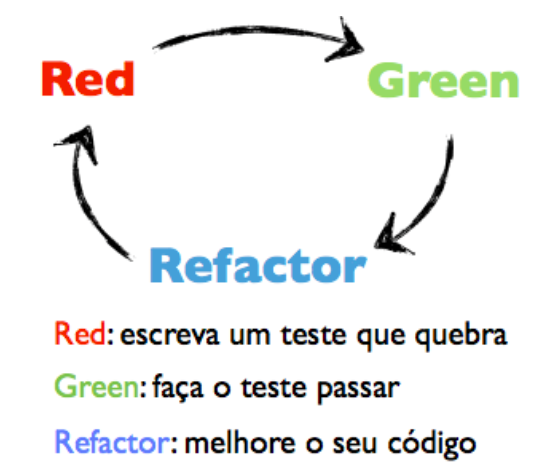
\includegraphics[width=9cm]{assets/tdd} \\
\fonte{\citeauthoronline{barauna:13}, \citeyear{barauna:13}.}
\end{center}
\end{figure}	

Outra abordagem para incorporar qualidade é o BDD (\textit{Behavior Driven Development}) que é uma evolução do TDD. O BDD começou como uma tentativa de melhor entender e explicar o processo do TDD. O problema era basicamente a palavra ``Teste'' no TDD que fazia com que os desenvolvedores não utilizassem o TDD como uma ferramente de \textit{design} ou projeto para o \textit{software}. Com o passar do tempo, o BDD evoluiu no sentido de testar o comportamento de um objeto ao invés de sua estrutura interna (como é o foco do TDD). \cite{chelimsky:12}


A Figura \ref{fig:bdd} ilustra o processo do BDD. Primeiramente o desenvolvedor descreve um cenário de teste. Após a escrita desse cenário, é escrita uma \textit{step-definition}, que descreve um comportamento de uma funcionalidade do sistema. Nessa \textit{step-definition}, o desenvolvedor escreve somente o um trecho de código necessário para o teste falhar. Após esse processo, entra-se num ciclo do BDD que foi mostrado anteriormente. Na linguagem ruby pode-se utilizar o Cucumber e o Rspec como \textit{frameworks} para BDD e TDD respectivamente.

\begin{figure}[htb!]
\begin{center}
\caption{Ciclo do BDD}
\label{fig:bdd}
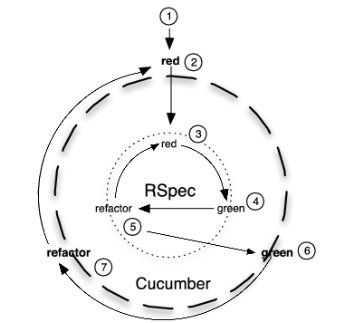
\includegraphics[width=9cm]{assets/bdd} \\
\fonte{\citeauthoronline{chelimsky:12}, \citeyear{chelimsky:12}.}
\end{center}
\end{figure}	

O trabalho do teste não pode-se limitar apenas a encontrar defeitos de produção no sistema e sim fazer  que os erros e problemas posssam ser previnidos e detectados para que não entrem em produção.

\subsection{Criar Conhecimento}

O conhecimento do desenvolvimento de \textit{software} não é criado em apenas uma etapa. Um dos problemas com o modelo de desenvolvimento em cascata (visto na sessão \ref{sec:cascata}) é que ele assume que todo conhecimento é adquirido na etapa de análise, porém a construção de um \textit{software} é um processo de criação de conhecimento. Mesmo que todos os detalhes sejam vistos na etapa de análise, os detalhes de \textit{design} sempre ocorrem na etapa de contrução (quando o \textit{software} está sendo codificado). Um processo de desenvolvimento que seja focado na criação de conhecimento deve esperar que o \textit{design} evolua durante a codificação, principalmente porque o cliente quase sempre não sabe o que quer, assim o \textit{feedbacks} dos \textit{stakeholders} são importantes nesse processo e dão direcionamento para o que está sendo elaborado.

As empresas que possuem excelência no desenvolvimento de \textit{software} aprendem no processo de construção do \textit{software} e utilizam o conhecimento aprendido para futuros projetos. O processo de desenvolvimento precisa encorajar o aprendizado através do ciclo de desenvolvimento. 


\subsection{Adiar Compromisso}

Um sistema de \textit{software} é passivel de sofrer mudanças: todos os requisitos e riscos dificilmente vão ser mitigados em uma primeira etapa de análise. Porém, toda e qualquer decisão que torne o processo de mudança mais difícil ou irreverssível deve ser postergada até o último momento. É melhor deixar uma decisão importante para o último momento do que tomar uma decisão prematura que não leve a lugar algum. Isso não significa que todas as decisões devem ser postergadas, o time ou o líder de tecnologia deve comprometer-se a fazer com que a maioria das decisões sejam reversíveis com um sistema e arquitetura que sejam o mais flexível possível. As vezes a pressa pela eliminação de riscos a fim de diminuir a incerteza pode levar a decisões erradas que são irreversíveis. O melhor a se fazer é experimentar várias soluções, deixando as opções em aberto para serem tomadas o mais tarde possível com os testes e avaliações necessários.

\subsection{Entregar rápido}

Todo desenvolvimento de \textit{software} deve ser feito da forma mais rápida possível para que o cliente não tenha tempo de mudar de ideia. Num mundo rápido e cada vez mais competitivo, a rapidez de implementação de uma ideia pode ser fundamental para seu sucesso. Isso pode ser conseguido através da eliminação do desperdício e gastos desnecessários, diminuição das taxas de erros (através de inspeções no código) etc.

A teoria das filas é uma teoria que pode ajudar nesse sentido. Muitas vezes no desenvolvimento há novas demandas de cliente ou defeitos para serem corrigidos e organizar essas é de certa maneira desafiador. A teoria das filas ajuda no gerenciamento dessa lista de ``requisitos''.

\subsection{Respeitar pessoas}

Três dos quatro pilares do sistema de desenvolvimento de produtos da Toyota dizem respeito as pessoas envolvidas no processo de desenvolvimento de um produto. Assim, esse é um princípio muito importante que norteia o desenvolvimento \textit{lean}.

As pessaos são motivadas a trabalharem em produtos de sucesso e para conseguir-se produtos de sucesso é necessário bons líderes. Empresas que respeitam seus empregados desenvolvem grandes líderes que por sua vez são capazes de conduzir grandes projetos. Além disso, é necessário assegurar-se que o conhecimento técnico necessário esteja presente na pessoa que designa a função. Distrubuir a pessoa de acordo com seu perfil e capacidade para um projeto é fundamental para o sucesso do projeto. O respeito as pessoas está relacionado com a capacidade do time em se organizar em relação aos planos e objetivos da empresa. Todas as pessoas precisam fazer parte do processo: isso envolve desenvolvedores, \textit{stakeholders} etc. O processo de construção de \textit{software} também é um processo de certa forma ``social''.

\subsection{Otimizar o todo}

Uma empresa que utiliza-se do \textit{lean} otimiza a cadaia de valor desde o princípio até seu final. Se algum processo dentro dessa cadeia não é otimizado, o processo como um todo é afetado. Aqui é feita uma análise do processo de desenvolvimento \textit{lean}, mas não adianta o processo de desenvolvimento ser otimizado, se outros processos que também fazem parte do processo de negócio apresentarem deficiência. Uma das ferramentas presentes e que foi mostrado no Capítulo 1 é a utilização de mapas de cadeia de valor. Através da análise da cadeia de valor é possível enxergar desperdícios com uma visão holistica de todo o processo da empresa. 

\section{DISCIPLINA, QUALIDADE e 5S}

No desenvolvimento de \textit{software} \textit{lean} não é possível acelerar o desenvolvimento sem incorporar qualidade no produto (como foi visto nos princípios do \textit{lean} acima). Para tornar-se \textit{lean} é indispensável que haja disciplina no que diz respeito a maneira como o \textit{software} é desenvolvido. Ao entrar em ambiente de desenvolvimento é possível perceber o nível de disciplina que uma equipe possui. Se a sala de desenvolvimento está bagunçada, possívelmente a equipe é desleixada, o que pode fazer com que o código também possua essa qualidade negativa. O Cinco S é uma ferramenta clássica do \textit{lean} que ajuda a organizar o espaço de trabalho de uma equipe garantindo que tudo que seja necessário esteja em mãoes no momento que a equipe precise. Os Cinco S são referências as palavras japonesas \textit{seiri, seiton, seiso, seiketsu e shitsuke}. Essas palavras foram traduzidas para a língua inglesa e são: \textit{sort} (organização), \textit{sistematize} (classificação), \textit{shine} (limpeza), \textit{standardize} (padronização) e \textit{sustain} (autodisciplina). No desenvolvimento de \textit{software}, o 5S não se aplica apenas ao ambiente físico, mas também ao ambiente lógico por trás da tela. Para organização poderia ser, por exemplo, remover e fazer \textit{backup} de códigos e arquivos que não são mais utilizados, para classificação envolve organizar as coisas nos servidores de forma que o ambiente possa ser utilizado por qualquer pessoa da empresa. Limpeza pode ser manter o ambiente de desenvolvimento limpo (sem copos, marcas de dedo na tela etc.). Padronização envolve, por exemplo, colocar automatização para garantir que cada estação de trabalho tenha a versão mais recente ou a que foi acordada para o desenvolvimento do produto, \textit{backup regular} etc. A autodisciplina só precisa ser então mantida no ambiente. 


Em \citeonline{poppendieck:07} é mostrado também os 5S em relação a linguagem Java, mas que serve para a programação em geral. Abaixo é mostrado cada S com sua respectiva ação para melhoria.

\subsection{Organização}
\label{lean:org}

A organização na linguagem Java envolve reduzir o tamanho do código do repositório. Para isso, é necessário eliminar tudo que for:

\begin{itemize}
	\item Códito morto (que não faz nada);
	\item Imports que não são utilizados;
	\item Variáveis que não são utilizadas;
	\item Métodos que não são utilizados;
	\item Classes que não são utilizadas e
	\item Refatorar códigos redundantes.
\end{itemize}

\subsection{Classificação}

A classificação ou sistematização envolve organizar o projeto e pacotes. Tudo precisa ter uma local e tudo precisa estar no seu devido lugar. Para isso é necessário:

\begin{itemize}
	\item Resolver ciclos de dependência de pacotes e
	\item Minimizar depenpências.
\end{itemize}

\subsection{Limpeza}

Os problemas são mais visíveis quando o código está limpo e claro. Para resolver problemas de limpeza pode-se executar as seguintes ações:

\begin{itemize}
	\item Resolver testes que estão falhando e erros;
	\item Melhorar cobertura de código;
	\item Melhorar performance de teste e
	\item Resolver os ``\textit{warnings}'' que aparecem no teste ou nos \textit{logs}.
\end{itemize}

\subsection{Padronizar}

Uma vez que o ambiente encontra-se limpo, deve-se mantê-lo asssim. Reduzir a complexidade é importante para melhorar o processo de manutenção. Uma técnica bastante utilizada para resolver questões desse tipo é médir o \textit{software}. Primeiramente é necessário saber o que medir e para quê. Esses dados são importantes e podem dar uma direção para equipe no que tange a qualidade do código. Uma técnica de medição, chamada de complexidade ciclomática pode ajudar segundo \citeonline{laird:06}. Quanto maior a complexidade do código, mais difícil é mantê-lo.

\subsection{Autodisciplina}

Para autodisciplina é necessário seguir e usar procedimentos.


\section{CONCLUSÃO DO CAPÍTULO}

Nesse capítulo foi visto sobre a metodologia \textit{lean} de desenvolvimento. O \textit{lean} foi uma metodologia de desenvolvimento que nasceu na manufatura e que hoje está cada vez mais sendo aplicada no \textit{software}. Foram visto os princípios do \textit{lean} como eliminação de desperdícios, incorporar qualidade, criar conhecimento, adiar compreomisso, entregar rápido, repeitar pessoas e otimizar o todo e como eles são aplicados no desenvolvimento. A importância de testes e detecção de falhas também foi explicada. Além disso, foi discutida a importância do mapeamento do fluxo de valor para uma empresa de forma a entender e eliminar os despedícios. Utilizar uma prática do \textit{lean} não necessáriamente vai tornar uma empresa \textit{lean} se os desperdícios não forem eliminados e o processo não for melhorado. Sem fazer esse mapeamento do fluxo de valor, não há como melhorar o processo. No próximo capítulo são mostradas algumas melhorias que foram identificas e até implementadas no que diz respeito aos princípios do \textit{lean}. 

\chapter{IMPLEMENTANDO LEAN EM UMA EMPRESA DE SOFTWARE}

Esse trabalho, como identificado na sessão \ref{chap1:obj}, tem como objetivo propor uma melhoria no modelo de desenvolvimento de uma empresa de \textit{software} aplicando conceitos do \textit{lean}. Assim, esse capítulo aborda o processo de desenvolvimento atual e tenta melhora-lo com alguns  dos princípios do desenvolvimento \textit{lean} de \textit{software} vistos no Capítulo \ref{cha:lean}.

\section{A EMPRESA}

Nesse capítulo é descrito o processo de desenvolvimento de uma empresa de \textit{software} do ramo de auto publicação de livros. O nome da empresa não é mencionado, mas isso não contribui de forma negativa para o trabalho proposto. A empresa possui atualmente três sistemas, os quais foram desenvolvidos utilizando-se a linguagem de programação ruby. Além da linguagem ruby, é utilizado o \textit{framework} Rails, já que os produtos são plataformas SAAS (\textit{Software as a Service}). Outras tecnologias utilizadas são: AWS (\textit{Amazon Web Services}), para armazenamento de arquivos e imagens na núvem, Postgres SQL (para banco de dados) e outras tecnologias. 

No que tange a equipe de desenvolvimento, a equipe foi composta até pouco tempo por três programadores, e hoje conta apenas com um engenhairo de \textit{software} que é responsável por atender solicitações do dono do negócio (ou \textit{Product Owner} no Scrum). Esse profissional é responsável pela parte de \textit{backend} (lógica de negócios), \textit{frontend} e suporte técnico (quando necessário). A análise técnica e estimativa também é feita por esse profissional. Um time de atendimento ao usuário (duas pessoas) também existe, o qual passa as demandas de suporte técnico (quando existem) via Zendesk (ferramenta de suporte). Alguns pontos de melhorias anteriores a esse trabalho contribuíram para a implantação do \textit{lean}, então essas melhorias também são mencionadas. A sessão seguinte mostra o processo utilizado atualmente.

\section{O PROCESSO DE SOFTWARE ATUAL}
\label{sec:processo_atual}

Para implementar o desenvolvimento \textit{lean} em uma empresa, como visto no capítulo anterior, é fundamental identificar e conhecer o processo de \textit{software} e identificar os desperdícios como visto na sessão \ref{sec:desperdicios}. Na Figura \ref{fig:processo_atual} é mostrado o fluxo básico da empresa atualmente. Tudo começa com o \textit{backlog} de produto. O \textit{backlog} de produto foi um componente tirado do Scrum (visto na sessão \ref{sec:scrum}). Atualmente utiliza-se um modelo de Scrum, mas sem algumas cerimônias como \textit{daily meeting}, já que todo o processo é feito hoje apenas por uma pessoa. O \textit{product owner} é responsável por colocar os itens e priorizar o \textit{backlog}. Através de uma reunião, os items são colocados em um \textit{backlog} de \textit{sprint}, que vão compor uma \textit{sprint} que dura de 2 até 3 semanas. Quando iniciada a \textit{sprint}, o desenvolvimento de uma funcionalidade vai seguir um modelo incremental: não necessáriamente em um ciclo a funcionalidade toda vai acabar. Cada vez que uma funcionalidade estiver pronta, pode-se enviar para o ambiente de homologação para os \textit{stakeholders} validarem e darem um \textit{feedback}. Testes efetuados por terceiros são feitos em projetos maiores (embora não estejam representados no processo). Caso a funcionalidade seja validada, ela pode ser enviada para produção. Quando todas as funcionalidades estiverem prontas, a \textit{sprint} termina.

\begin{figure}[htb!]
\begin{center}
\caption{Processo de desenvolvimento atual com desperdício identificado}
\label{fig:processo_atual}
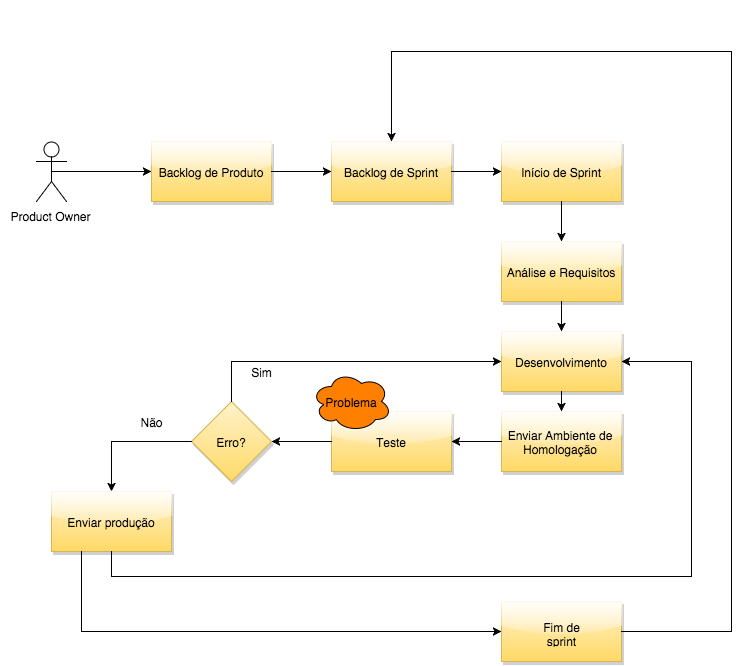
\includegraphics[width=12cm]{assets/compreender_problema} \\
\fonte{Autoria própria}
\end{center}
\end{figure}


\section{IDENTIFICANDO DESPERDÍCIOS}
\label{sec:identificando_despercio}

Um dos problemas apontados na Figura \ref{fig:processo_atual} da sessão \ref{sec:processo_atual} é apontado na nuvem identificada com a palavra ``problema''. O sistema principal da empresa, que está em foco nesse trabalho e representa mais de 80\% da renda da empresa, foi construido sem as técnicas apresentadas na sessão \ref{sec:quality} como TDD e BDD. Toda vez que uma alteração no sistema precisa ser feita, não há como prever se alguma funcionalidade existente pode ser afetada. Se o sistema fosse construído com o uso de TDD e BDD, os testes seriam rodadas em cada \textit{deploy}, e caso algum comportamento do sistema falhasse, o código teria que ser reescreito, o que evitaria de enviar novos problemas para produção. Esse tipo de problema fere claramente o princípio da eliminação de desperdício e da incorporação de qualidade. No \textit{lean}, como visto no Capítulo \ref{cha:lean}, é preciso não apenas garantir o teste depois da codificação, mas trabalhar na questão de detecção do erro. Em uma analogia com o sistema Toyota de manufatura, toda vez que houver algum problema na linha de produção, esse problema deve ser detectado e a linha de produção deve parar para que o problema ou defeito seja corrigido. Uma das maneiras de se identificar esses desperdícios é montando o fluxo da empresa em um gráfico que pode ser um diagrama de fluxo de valor como mostra a Figura \ref{fig:01} no Capítulo \ref{chap:01} ou de forma mais simples como identificado na Figura \ref{fig:processo_atual}.

\section{RESOLVENDO DESPERDÍCIO}

Como mencionado na sessão \ref{sec:identificando_despercio}, existe um problema que faz com que novos suportes e \textit{tickets} no Zendesk sejam frequentes cada vez que uma ou mais novas funcionalidades entrem no ar. Devido a complexidade do sistema, é praticamente impossível e até mesmo inviável (devido a presença de apenas uma pessoa na equipe) que se teste o sistema inteiro sempre que uma nova funcionalidade seja enviada para o ambiente de produção. Mas qual a melhor alternativa para resolver problemas de teste em sistemas legados com nenhuma cobertura de testes ? 

\begin{figure}[htb!]
\begin{center}
\caption{Tipos de testes}
\label{fig:tipo_testes}
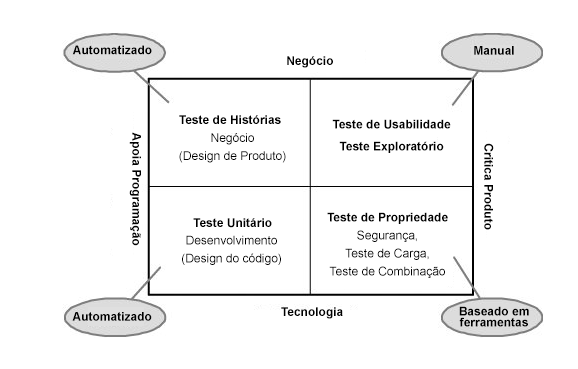
\includegraphics[width=14cm]{assets/testetab} \\
\fonte{\citeauthoronline{poppendieck:07}, \citeyear{poppendieck:07}.}
\end{center}
\end{figure}

A Figura \ref{fig:tipo_testes} mostra os tipos de testes existentes e suas finalidades. Como pode-se observar, os testes podem estar mais relacionados com questões de negócio ou tecnológicas. Ao mesmo tempo ele pode apoiar mais a programação em si ou fazer críticas ao \textit{software}. Um teste de usabilidade (relacionado ao segundo quadrante superior), por exemplo, poderia encontrar problemas relacionados a dificuldade de se encontrar alguma coisa na tela, ou a realizar alguma ação etc. Esse tipo de testes geralmente é executado por alguma pessoa, e já é realizado na empresa. Os testes de negócio e unitários foram descritos na sessão \ref{sec:quality}. Os testes de propriedade podem testar questões relacionadas a segurança do sistema, carga e combinação. Frequentemente pode-se utilizar ferramentas prontas para, por exemplo, achar vulnerabilidades conhecidas em códigos, pastas com permissões indevidas etc. Um exemplo desse tipo de ferramente de teste de propriedade é o WPSCan\footnote{O WPScan pode ser encontrado e baixado no endereço http://bit.ly/1MPrh2w.}, que procura vulnerabilidades em um sistema feito com Wordpress.

No caso do sistema da empresa em questão, é importante garantir que as novas funcionalidades sejam feitas utilizando-se do princípio do TDD e BDD, pois ele garante que o desenvolvimento seja maduro através do processo de \textit{design} do código e da refatoração, que se encaixa no \textit{seiri} (organização) no 5S do \textit{lean}. Em casos como esse, em que há pouca cobertura de teste, é preciso saber o que testar. Nesse caso, é indispensável que funcionalidades essenciais do sistema estejam coberta por testes.

Como mencionado no início do capítulo, o sistema da empresa foi implementado com o \textit{framework} Rails. Houve uma demanda do suporte de mudança no cadastro de usuários: que é uma parte crítica do sistema. Basicamente a ficha cadastral foi combinada com outra ficha de cadastro relacionada aos autores (que antes era separada). Uma das maneiras de se testar que tudo sempre vai funcionar como esperado é implementar teste de \textit{views}. Utilizando o \textit{Selenium Web Browser} com uma ferramenta chamada Capybara\footnote{O projeto Capybara pode ser encontrado no endereço http://bit.ly/1ht90TA.}, que torna a escrita de testes que utilizam-se do Selenium mais fácil, foi possível escrever testes que são codificados uma vez e que vão executar automaticamente de forma lógica. 

\begin{figure}[htb!]
\begin{center}
\caption{Teste de \textit{View}}
\label{fig:teste_view}
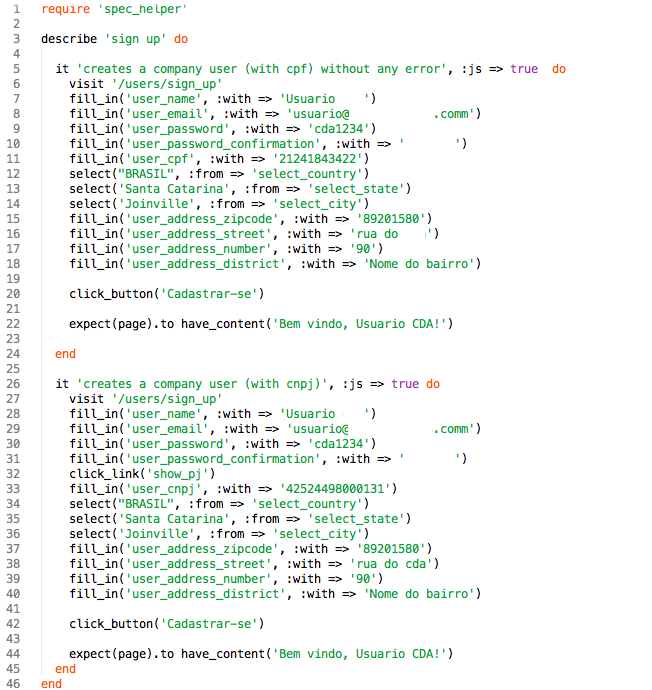
\includegraphics[width=15cm]{assets/teste_view} \\
\fonte{Autoria própria.}
\end{center}
\end{figure}

A Figura \ref{fig:teste_view} mostra um teste de \textit{view} para o cadastro. Basicamente ele testa a criação de um usuário normal sem erro algum e a criação de um usuário do tipo pessoa jurídica sem erro algum. Como o sistema trata da criação de autores também, que podem ser pessoa física ou jurídica, os testes para esses casos também devem ser implementados. Ao final deve haver os seguintes testes: pessoa física não autora, pessoa física autora, pessoa jurídica não autora e pessoa jurídica autora.

Ao rodar os testes, o \textit{browser} abrirá e os dois casos são testados. Caso o comportamente no bloco expect não aconteça, o teste falhará.

Esse tipo de abordagem e teste demonstra ser interessante em sistemas legados e com poucos teste, pois futuramente não precisa se gastar tempo testando manualmente se uma dada funcionalidade do sistema está funcionando ou não. Esse código ainda pode ser melhorado para eliminar duplicidade (conforme o \textit{seiso} ou limpeza do 5S). Muitos campos estão sendo testados com o mesmo nome, logo eles poderiam estar numa função que é chamada antes de entrar em cada bloco it.

Outra forma de incorporar qualidade no serviço é utiliza-se de ferramentas de métricas que avaliam a complexidade do código e ferramentas que analisam os erros que ocorrem em ambiente de produção. Uma ferramenta desse tipo pode ser o Airbrake, que é mostrada na Figura \ref{fig:airbrake}. Caso aconteça algum erro em algum ambiente, a empresa é notificada e pode tomar alguma ação antes de receber uma reclamação ou que alguma coisa mais séria aconteça. Programas que avaliam métrica do sistema como complexidade cicliomática, podem indicar locais do código com alta complexidade, e que possivelmente são mais difíceis de serem mantidos ou que possuem algum erro.

\begin{figure}[htb!]
\begin{center}
\caption{Ferramenta de detecção de bugs}
\label{fig:airbrake}
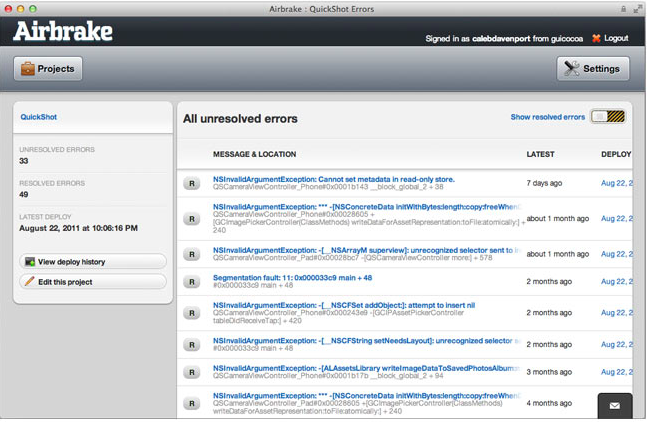
\includegraphics[width=15cm]{assets/airbrake} \\
\fonte{Autoria própria.}
\end{center}
\end{figure}

\section{ORGANIZANDO O TRABALHO}

Um componente muito utilizado pelas empresas, e que foi implantado de modo eletrônico, vindo do \textit{lean} foi o Kanban. Segundo \citeonline{poppendieck:10}, a palavra kanban significa cartão e é utilizada na manufatura para indicar o trabalho que precisa ser feito. O kanban pode ser utilizado no desenvolvimento de \textit{software} para indicar o andamento de uma funcionalidade no fluxo de produção. Para o \textit{kanban}, há uma coluna para cada passo dentro do fluxo de trabalho da empresa. Tudo isso pode ser feito em nível mais abrangente, como as histórias de usuário, como mais técnicos como as implementações necessárias para uma funcionalidade.

Os sistemas de \textit{kanban} são projetados para limitar o trabalho que está sendo executado, pois quanto mais processos estão sendo executados, mais lento é o fluxo de trabalho. Essa é a principal razão da invenção do \textit{kanban}, segundo \citeonline{poppendieck:10}, ou seja limitar o trabalho que está sendo executado e melhorar o fluxo no processo. A Figura \ref{fig:kanban} mostra um exemplo de um quadro. Cada coluna representa um passo, ou etapa no fluxo de trabalho de uma empresa. No exemplo da figura cada funcionalidade chega ao quadro pelo lado esquerdo na coluna ``\textit{Next Features}''. O número máximo de funcionalidades que devem ficar nessa coluna são três. Quando há  espaço suficiente, a funcionalidade muda de estado. No próxima etapa, a funcionalidade é decomposta em histórias e depois são postas na próxima coluna. O fluxo segue através do desenvolvimento e testes unitários e depois para o teste de aceitação. Uma vez que uma funcionalidade passe no teste de aceitação, elas são transformadas em funcionalidades novamente e passam pelo teste de aceitação de funcionalidade e \textit{staging}. Finalmente, a funcionalidade é colocado na coluna de pronto (\textit{Ready to Release}).

O membro do time pode trabalhar em qualquer etapa que tiver habilidade. Quando uma funcionalidade termina, o tempo para que ela se movesse através do quadro de \textit{kanban} é anotado. O dia em que a funcionalidade foi posta em ``\textit{Next Features}'' é subtraído do dia em que ela entrou em ``\textit{Ready to Release}''. O resultado é então colocado no gráfico ``\textit{Days to Complete Feature}'' (dias para completar a funcionalidade).

\begin{figure}[htb!]
\begin{center}
\caption{Exemplo de um kabban}
\label{fig:kanban}
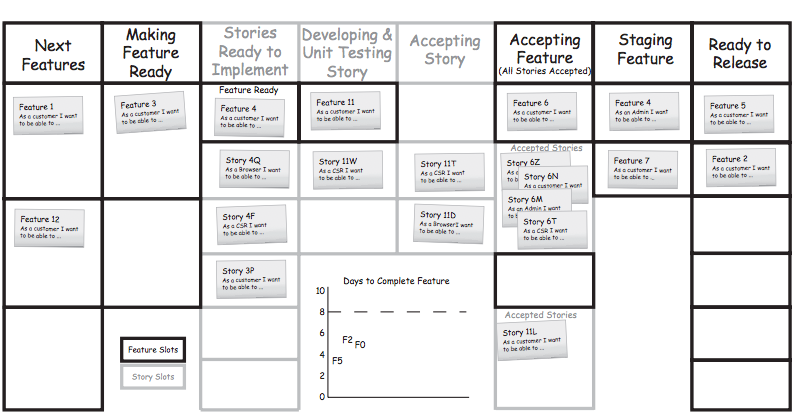
\includegraphics[width=14cm]{assets/kanban} \\
\fonte{\citeauthoronline{poppendieck:10}, \citeyear{poppendieck:10}.}
\end{center}
\end{figure}

Existem outras variações do \textit{kanban} e na empresa foi implementada uma versão eletrônica utilizando-se da ferramenta Trello\footnote{O trello é uma ferramenta livre e pode ser utilizado através do endereço http://bit.ly/1eyOBPE}. Na empresa, foi utilizado os seguintes passos (para uma funcionalidade), To--Do, Em Execução, Feito e parado. Algumas informações forem omitidas na imagem para preservar a empresa. O exemplo do \textit{kanban} pode ser visto na Figura \ref{fig:trello}.

\begin{figure}[htb!]
\begin{center}
\caption{Exemplo de kabban na empresa}
\label{fig:trello}
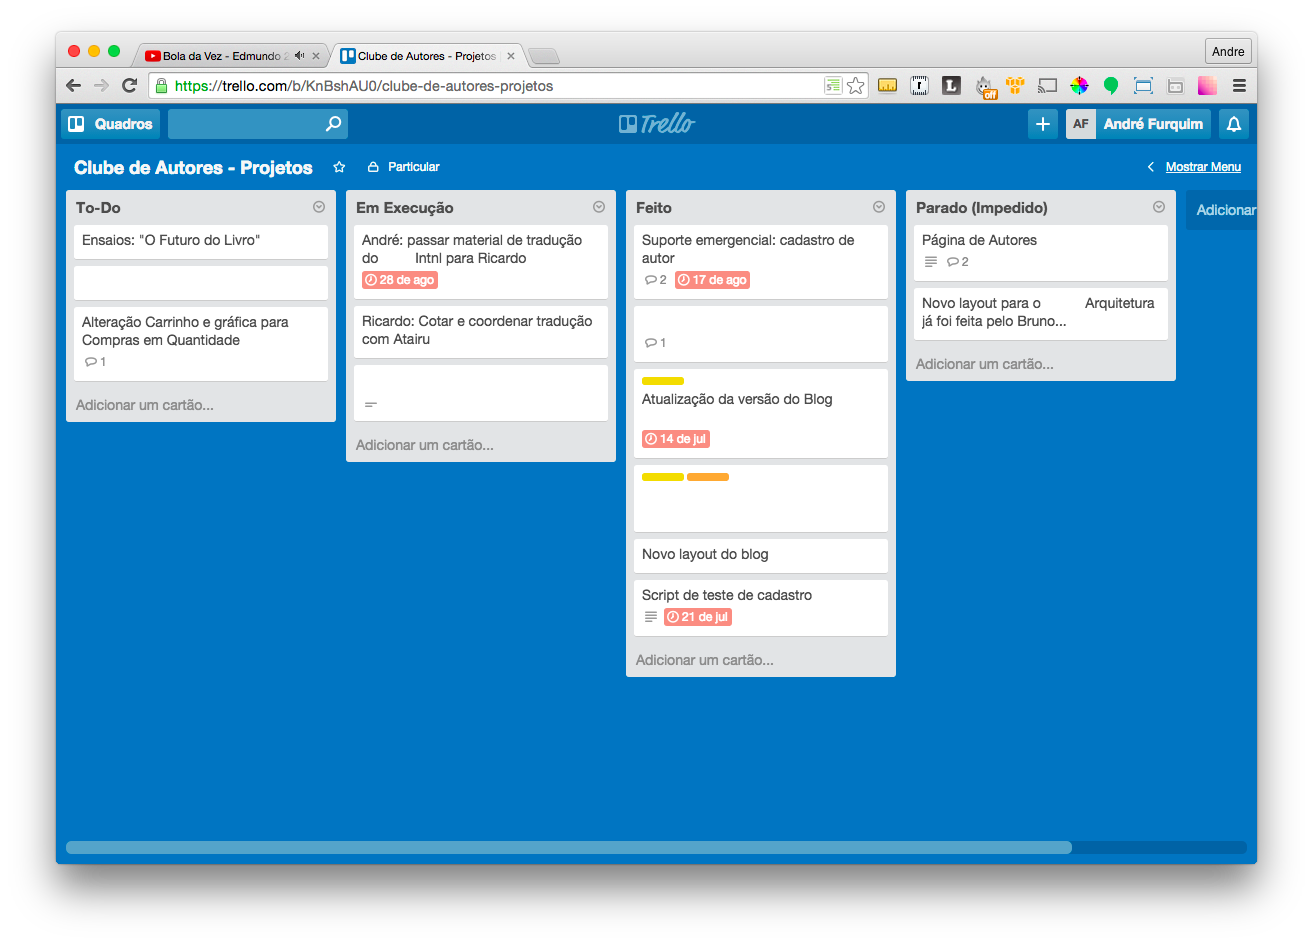
\includegraphics[width=14cm]{assets/trello} \\
\fonte{Autoria própria.}
\end{center}
\end{figure}

\section{CONCLUSÃO DO CAPÍTULO}

Nesse capítulo foram vistos alguns problemas da empresa e suas soluções aplicando os princípios \textit{lean} de desenvolvimento de \textit{software}. Foi visto que algumas demandas de suporte foram diminuidas através da utilização de teste não apenas depois da implementação de uma funcionalidade, para ver se tudo funciona conforme o desenvolvimento, mas de maneira preventiva ou trabalhando-se na sua detecção. Para melhorar o processo da empresa é fundamental que seja entendido o seu fluxo e que seus desperdícios sejam eliminados. Existe várias outras técnicas, em nível de programação, que também pode auxiliar no processo e que acabaram sendo incorporadas e que foram identificadas na sessão \ref{lean:org}. No próximo capítulo é feita a conclusão sobre o trabalho realizado.
% \section{OBJETIVOS}
% \label{chap1:obj}
% O objetivo deste trabalho é propor uma metodologia de aplicação do \textit{lean} em uma empresa de \textit{software} que já utiliza-se de algumas práticas ágeis. Assim, é necessário identificar pontos falhos no modelo de desenvolimento da empresa para melhorar os projetos.
% Para elaborar esse modelo, algumas perguntas precisam ser antes respondidas como:
% \begin{itemize}
% 	\item Como aplicar \textit{lean} no ambiente de desenvolvimento ?
% 	\item Existe uma formula que possa ser aplicada para qualquer empresa ?
% 	\item O quanto as práticas atuais da empresa estão perto ou longe do melhor cenário possível para o \textit{lean} ?
% 	\item Quais ferramentas de \textit{software} podem auxiliar o processo ?
% \end{itemize}
% Ao longo desse trabalho, essas perguntas são respondidas.
% \subsection{Objetivos Específicos}
% Afim de melhorar o ciclo de desenvolvimento, é necessário eliminar os desperdícios (um dos princípios do \textit{lean}). Assim é necessário:
% \begin{itemize}
% \item representar o modelo atual de desenvolvimento de uma maneira que fique bem claro para as pessoas envolvida, tanto a nível de negócio como operacional, os problemas existente; 
% \item Propor um novo modelo, que elimine esses desperdícios e
% \item Sugerir ferramentas que possam melhorar o processo de desenvolvimento.
% \end{itemize}

\chapter{CONCLUSÃO}
\label{chap:conclusao}

Esse trabalho teve como objetivo aplicar métodos de desenvolvimento \textit{lean} em uma empresa de \textit{software}. Através da aplicação de alguns desses princípios, foi notado uma melhora significativa no que tange a manutenção do sistema assim como nos \textit{tickets} recebidos de problemas de suporte relacionado a funcionalidade do teste em questão. 

Para entender e melhorar o processo de desenvolvimento de uma empresa foi importante estudar as diferentes metodologias e suas práticas, como por exemplo o TDD no \textit{Extreme Programming}, vistos no Capítulo \ref{cap:02}. Para se aplicar o \textit{lean} em uma empresa de desenvolvimento não existe uma fórmula correta, pois tudo vai depender da empresa e do negócio. Utilizar-se dos princípios do \textit{lean}, como \textit{kanban} por exemplo, não necessariamente vai ajudar a empresa a eliminar desperdício ou melhorar sua organização. Além de tudo, o desenvolvimento é feito por pessoas e investir na equipe e entender as necessidades da pessoa é fundamental para qualquer projeto.

Para se aplicar \textit{lean} em uma empresa de \textit{software} é necessário entender o desenvolvimento, a equipe e todas as pessoas envolvidas e contrastar com os seus princípios e perguntar-se ``Qual é a melhor maneira de eliminar esse desperdício?''. Práticas como TDD, BDD, \textit{clean code} etc., sem dúvida melhoram o desenvolvimento e qualidade do \textit{software} e vem se tornando um padrão na indústria de desenvolvimento para incorporar qualidade no sistema.


\section{Trabalhos Fufutos}

Os seguinte trabalhos futuros podem ser implementados para a conformidade com o desenvolvimento \textit{lean} e até na área do \textit{lean}:

\begin{itemize}
	\item Implementar integração contínua nos produtos da empresa;
	\item Desenvolver um manual de práticas de codificação com práticas de desenvolvimento para uma empresa;
	\item Aprimorar ainda mais as técnicas de desenvolvimento do \textit{lean} com o desenvolvimento da empresa e
	\item Implementar um modelo para gerenciamento do conhecimento na empresa conforme o princípio do \textit{lean}.
\end{itemize}


\postextual


\bibliography{referencias}

%% Referencias. LISTAR EXATAMENTE AS CITADAS NO TRABALHO.
% \begin{thebibliography}{99}

% %% ALGUNS EXEMPLOS ABAIXO

% \bibitem{Ferrari2003} FERRARI, M. Amplia\c{c}\~ao e refor\c{c}o do vocabul\'ario em l\'ingua estrangeira atrav\'es da narra\c{c}\~ao e 
% da leitura de hist\'orias infanto-juvenis. \textit{Letras Hoje}, Porto Alegre, v. 39, n. 3, p. 73-90, set. 2003.

% \bibitem{CalcB} FLEMMING, D. M.; GON\c{C}ALVES, M. B. \textit{C\'alculo B.} S\~ao Paulo: Makron Books, 2007.

% \bibitem{Figueiredo96} FIGUEIREDO, D. G. \textit{An\'alise I.} Rio de Janeiro: Livros T\'ecnicos e Cient\'ificos, 1996.

% \end{thebibliography}




%% Apendices

% \begin{apendicesenv}

% \chapter{T\'itulo do Primeiro Ap\^endice}

% ``Texto ou documento elaborado pelo autor, a fim de complementar sua argumenta\c{c}\~ao, 
% sem preju\'izo da unidade nuclear do trabalho''
% (ASSOCIA\c{C}\~AO BRASILEIRA DE NORMAS T\'ECNICAS, 2011, p. 6).

% ``Elemento opcional. Deve ser precedido da palavra \textbf{AP\^ENDICE}, identificado por letras mai\'usculas 
% consecutivas, travess\~ao e pelo respectivo t\'itulo. Utilizam-se letras mai\'usculas dobradas, 
% na identifica\c{c}\~ao dos ap\^endices, quando esgotadas as letras do alfabe\-to.''
% (ASSOCIA\c{C}\~AO BRASILEIRA DE NORMAS T\'ECNICAS, 2011, p. 13)
% \newline
% EXEMPLO:
% \begin{center}
% \textbf{AP\^ENDICE A - Avalia\c{c}\~ao num\'erica de c\'elulas inflamat\'orias}
% \end{center}


% \chapter{Segundo Ap\^endice}
% Texto do Segundo Ap\^endice 
% \end{apendicesenv}

%% Anexos

% \begin{anexosenv}

% \chapter{T\'itulo do Primeiro Anexo}
% ``Texto ou documento n\~ao elaborado pelo autor, que serve de fundamenta\c{c}\~ao, 
% comprova\c{c}\~ao e ilustra\c{c}\~ao''
% (ASSOCIA\c{C}\~AO BRASILEIRA DE NORMAS T\'ECNICAS, 2011, p. 9).

% ``Elementos opcional. Deve ser precedido da palavra \textbf{ANEXO}, identificado por letras mai\'usculas 
% consecutivas, travess\~ao e pelo respectivo t\'itulo. Utilizam-se letras mai\'usculas dobradas, 
% na identifica\c{c}\~ao dos anexos, quando esgotadas as letras do alfabeto.''
% (ASSOCIA\c{C}\~AO BRASILEIRA DE NORMAS T\'ECNICAS, 2011, p. 6).
% \newline
% EXEMPLO: 
% \begin{center}
% \textbf{ANEXO A - Representa\c{c}\~ao gr\'afica da contagem de c\'elulas inflamat\'orias presentes
% nas caudas em regenera\c{c}\~ao - Grupos de controle I (Temperatura)}
% \end{center}


% \chapter{T\'itulo do Segundo Anexo}
% Texto do Segundo Anexo


% \end{anexosenv}

%%% ---
\end{document}
